\chapter{Path Planning} \label{ch:pp}
The goal of each of the planners introduced is to assist in the discovery of a field's features with an adjustable trade off between speed and confidence of prediction. The user of such a system could choose to scan more area if fuel is not of high concern. Likewise, if the field is very large, or several fields need to be scanned in a limited amount of time, a quicker scan with a lower degree of prediction certainty can be performed.

\section{Vehicle \& Information Gain Model}
In an effort to formalize the dynamics of the exploration vehicle, and the information gain on the field, the models for vehicle dynamics and field variances will be introduced.

\subsection{Exploration Vehicle Model Dynamics} \label{sec:vehicledynamics}
The state vector of the vehicle will be defined as follows:
\begin{equation}
\vect{X} = \begin{bmatrix}
	x \\
	y \\
	\theta \\
	V
\end{bmatrix}
\label{eq:vehiclemodel}
\end{equation}

\noindent where $x$ and $y$ are the vehicle's position on a field, $\theta$ is the vehicle's heading angle, $\omega$ is the vehicle's angular velocity, $\dot{\theta}$, and $V$ is the magnitude of the linear velocity of the vehicle. Both $\omega$ and $V$ are control inputs to the vehicle.

The exploration vehicle dynamics will be modeled after a simple forward discrete kinematics model with a constant time step per iteration, $\Delta T$. An iteration of the propagation model will be the sum of the previous iteration, $\vect{X}_{k}$, the nonlinear vehicle dynamics, $\vect{f}(\vect{X}_k)$, and the control input, $\vect{u}_k$.

\begin{equation}
	\vect{X}_{k+1} = \vect{X}_k + \vect{f}(\vect{X}_{k}) + \vect{u}_k
	\label{eq:vehicledynamicsform}
\end{equation}

\begin{equation}
	\vect{X}_{k+1} = \vect{X}_k + \begin{bmatrix}
		V_k \Delta T \cos \theta_k \\
		V_k \Delta T \sin \theta_k \\
		0 \\
		0
	\end{bmatrix} + \begin{bmatrix}
	0 \\
	0 \\
	\theta_k \\
	V_k
	\end{bmatrix}
	\label{eq:vehicledynamicsmodel}
\end{equation}

The speed, $V$, is assumed to be regulated at a constant value for all values of $k$.

\subsection{Field Uncertainty Model} \label{sec:fielduncert}
In Section \ref{sec:krigvar}, a method for calculating the variance of a prediction was defined as a function of the proximity vector and Kriging weights generated for the prediction point. For points that have been directly measured, the variance is ideally zero (for fields with no drift or dynamics). The uncertainty of the prediction of a point in the target field is directly proportional to the variance of its prediction. The goal of a path planner intending to suppress uncertainty of predictions in a target field would be to reduced the overall variance of the target field being explored.

A criterion for overall field uncertainty can be defined as the average variance, calculated from a prediction of a target field from a set $S$ points sampled for all $h\times w$ predictable points on a target field.

\begin{equation}
	\Sigma(\hat{Z}_{S}) = \frac{1}{hw}\sum_{i = 1}^{hw} \text{var}\{\hat{Z}(\vect{p}_i)\}
	\label{eq:fielduncert}
\end{equation}

\subsection{Uncertainty Loss Function} \label{sec:lossfunc}
In Section \ref{sec:fielduncert}, a criterion for overall field uncertainty was introduced. Given a set of sampled points, $S$ on a field, the overall field uncertainty is the mean variance of all points on the field, $\Sigma(\hat{Z}_{S})$. For an additional set of samples, $T$, taken on the field, a new field uncertainty, $\Sigma(\hat{Z}_{S \cup T})$, is the field uncertainty criterion of the fields prediction from the union of the sample sets $S$ and $T$. The difference in overall field uncertainty, $L(T)$, will be defined as the uncertainty lost by taking the additional samples in the set $T$ on the field.

\begin{equation}
	L(T) = \Sigma(\hat{Z}_{S}) - \Sigma(\hat{Z}_{S \cup T})
	\label{eq:lossfunc}
\end{equation}

% The optimal path, $O$, subject to a limited scanning time constraint, is the path that simultaneously maximizes $L(S,O)$, and minimizes the length of of the path taken (using the assumption of a constant linear velocity from Section \ref{sec:vehicledynamics}).

% \begin{equation}
% 	O = \argmax_T\ \beta L(T) - (1-\beta)l(S + T)
% \end{equation}

% \noindent where $\beta \in [0,1]$ is a real number which puts more emphasis on exploration time over prediction quality. It is important to note that as more samples are taken, the overall field prediction variances change. It would be in the benefit of a path planner to batch process a set of points after meeting a predetermined waypoint, or after a threshold number of samples. 

% Given an endpoint in a single trajectory, in the limit, recalculating $O$ at every sample would optimally shape the trajectory of the exploration vehicle. With no endpoint selected, the exploration vehicle could be found in a repeating state due to being stuck in a global minimum in the variance field. In an effort to avoid the sticking minimum problem, the path planners introduced will be endpoint oriented (where the endpoint of any trajectory is predetermined), and the goal of each path taken is to make it to the endpoint. Furthermore, a new path will only be calculated as a batch process after sampling a trajectory. This is done in an attempt to reduce computation time as the Kriging predictions and variance calculations become more expensive as more samples are taken.

% \section{Finding Points of Highest Uncertainty} \label{sec:highestvars}
% Points on a target field with high prediction uncertainties should be sampled in order to reduce overall field uncertainty. After sampling an initial set of points, and then running a Kriging prediction on all points on a target, the variance of prediction of all points can be calculated.

% The motivation of the path finders introduced is to minimize the average uncertainty of a target field by sampling the points representing the highest prediction variances on the field. A set of points where the highest uncertainties lie are found on the field using a simple search.

% Let $S_k$ be a singleton set containing the point of highest variance on the $k^{th}$ iteration of the target field prediction variances, represented as the set $\text{var}\{\hat{Z}_k\}$, where $\text{var}\{\hat{Z}\} : \mathbb{R}^2 \to \mathbb{R}^+$.

% \begin{equation}
% 	S_{k} = \argmax_{\vect{s}} \ \text{var}\{\hat{Z}_{k}(\vect{s})\}
% 	\label{eq:highestvar}
% \end{equation}

% \noindent The cardinality of the set $S_k$ can be greater than one if there exist multiple instances of the same value of variance in the target field prediction variances. For the sake of simplicity, only the singleton case will be considered.

% Let $\text{var}\{\hat{Z}_{k+1}\}$ be the set of points, not including the point of highest variance found in the $k^{th}$ iteration of the set configuration (Equation \ref{eq:highestvar}), on a target field prediction.

% \begin{equation}
% 	\text{var}\{\hat{Z}_{k+1}(\vect{s})\} = \text{var}\{\hat{Z}_k(\vect{s})\} - S_k \\
% 	\label{eq:nextmaxvarsset}
% \end{equation}

% \noindent Let $S_{v}$ be the set of the $N$ points of highest uncertainty on the target field prediction variances, $\text{var}\{\hat{Z}\}$.

% \begin{equation}
% 	\label{eq:highestvarsunion}
% 	S_{v} = \bigcup_{k = 1}^{N} S_k = \bigcup_{k = 1}^{N} \text{var}\{\hat{Z}_k(\vect{s})\} - \text{var}\{\hat{Z}_{k+1}(\vect{s})\}
% \end{equation}

\section{Next Highest Variance Path Planner} \label{sec:nhvpp}
Sampling the location of the next highest variance (NHV) is the simplest and most naive approach to path planning using the Kriging method. The highest point of uncertainty on the field is the point, $\vect{p}$, is defined as:

\begin{equation}
\argmax_{\vect{p}} \ \text{var}\{\hat{Z}(\vect{p})\}
\end{equation}

By simply setting the next endpoint of the path to $\vect{p}$, the point of highest uncertainty will be sampled at the end of the path. Once the point is met at the end of the path, a new set of samples gathered from the path to the endpoint will be used to recalculate the statistical patterns of the field to higher degree of quality. A Kriging prediction, variances of those predictions are then run on the field. The path planner continues by setting the next endpoint to the next point of highest uncertainty after recalculating the variances of the field. The planner terminates exploration once a preset maximum scan area limit has been met by the exploration vehicle. An initial forward diagonal sweep of samples are taken across the field to generate an initial variogram and Kriging prediction variances before the path planner chooses its first endpoint.

\begin{figure}[hb!]
	\centering
	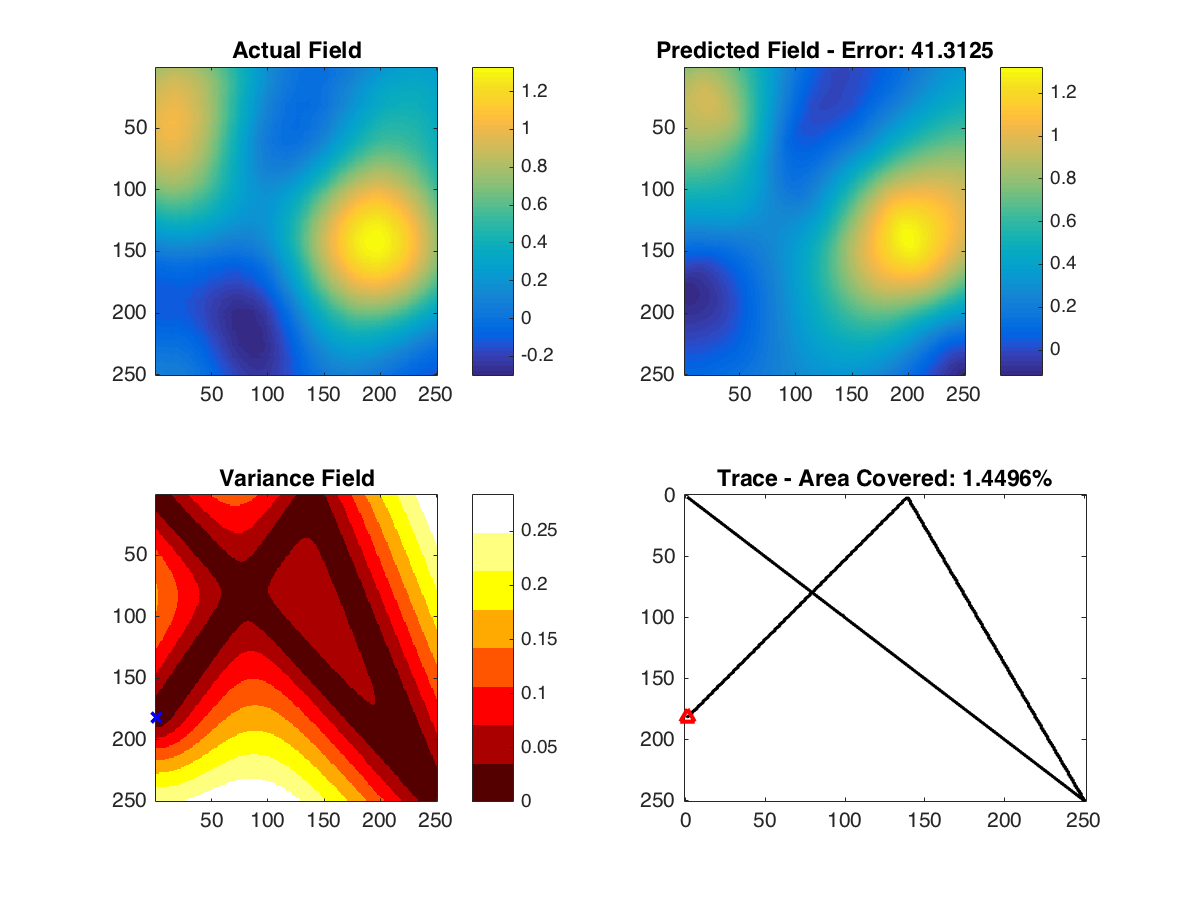
\includegraphics[width=0.95\linewidth]{figures/nhv_4panel.png}
    \captionsetup{skip=0.20\baselineskip}
	\ssp
	\caption{The Next Highest Variance (NHV) algorithm terminated after two iterations of the algorithm. The actual field that is being explored is shown in the upper left figure panel. The current prediction of the actual field is shown in the upper right. The variance of the current prediction of the field is shown in the lower left. The trace of the exploration vehicle's path taken to the point of termination (in red) is shown in the lower right panel. All distance units are in meters.}
	\label{fig:nhvpp}
\end{figure}

\subsection{Inefficiency in NHV}
The NHV algorithm does not account for repeating paths, or avoiding the re-sampling of points on the field. The only knowledge used is the variance of the endpoint of a path. Although the ground covered by the algorithm may be sufficient for uncertainty suppression, a path planner that considers the cost of trajectories would likely yield better results.

\section{$N$ Next Highest Variances Path Planner} \label{sec:nnhv}
A modification to the NHV algorithm can be made to consider more trajectories, and therefore compare the loss of taking a path from a set of possible paths. Let $K_N$ be the set of the $N \in \mathbb{N}$ points of highest uncertainty on the field. Let $T_i$ be a candidate trajectory connecting the current position of the exploration vehicle to the $i^{th}$ point in the set $K_N$. The endpoint that is ultimately chosen by the $N$ Next Highest Variance (N-NHV) Path Planner is the one that maximizes the loss function, $L(T_i)$. The points along a trajectory, $T_i$, have likely not been sampled, as they represent points of high uncertainty. The loss in uncertainty for taking the path, $T_i$, is therefore not known. An estimate of the loss in overall field uncertainty, $\hat{L}(T_i)$, after taking the path, $T_i$, is calculated by using the previous Kriging predictions of the points along the path. The predictions of those points are used as actual samples taken on the field in a new Kriging prediction variance calculation of the field. An initial forward diagonal sweep of samples are taken across the field to generate an initial variogram, initial Kriging predictions, and initial Kriging prediction variances before the path planner chooses its first endpoint.

% \begin{figure}[hb!]
% 	\centering
% 	\includegraphics[width=0.95\linewidth]{figures/nnhv_4panel.png}
%     \captionsetup{skip=0.20\baselineskip}
% 	\ssp
% 	\caption{The $N$ Next Highest Variance (N-NHV) algorithm (Section \ref{sec:nnhv} terminated after two iterations of the algorithm. The actual field that is being explored is shown in the upper left. The current prediction of the actual field is shown in the upper right. The variance of the current prediction of the field is shown in the lower left. The trace of the exploration vehicle's path taken to the point of termination (in red) is shown in the lower right panel. All distance units are in meters. Here, $N$, the number of endpoints selected is $N=3$.}
% 	\label{fig:nnhv}
% \end{figure}

\section{Monte Carlo Path Planner} \label{sec:mcpp}
By introducing noise into each of the trajectories found in the N-NHV path planner, a more optimal path can be found. Similarly to the N-NHV method, the Monte Carlo path that maximizes the loss of the overall field uncertainty is chosen as the next vehicle path. Let $K_N$ be the set of the $N$ points of highest prediction variances on the field. Let $T_i$ be a candidate trajectory from the current position of the exploration vehicle to the $i^{th}$ endpoint in $K_N$. Each point in the candidate trajectory is a waypoint the exploration vehicle will visit on its way to the last point in the sequence. The trajectory is a set of state vectors representing the field horizontal position, $x$, the field vertical position, $y$, and the vehicle heading angle, $theta$. The $k^{th}$ vector in the state candidate trajectory set, $T_i$, denoted as $T_{i}(k)$, will be the state the exploration vehicle will take on at that position on the field, i.e.

\begin{equation}
T_{i}(k) = \begin{bmatrix} x_i(k) \\ y_i(k) \\ \theta_i(k) \end{bmatrix}
\end{equation}

Let $\alpha \in \mathbb{R}$ be the step size of the vehicle from one point to the next within the trajectory, $T_i$. Let $\vect{w}_i \in \mathbb{R}^2$ be a vector of two zero-mean Wiener processes with a tunable process standard deviation which is less than the step size, $\alpha$. Furthermore, the step size of the vehicle, $\alpha$, can not be a value less than the distance the exploration vehicle can travel in one time-step, $\Delta T$, given a constant vehicle velocity of $V$.

\begin{equation}
\text{var}\{\vect{w}_i\} = \begin{bmatrix} \text{var}\{w_{i_x}\} \\ \text{var}\{w_{i_y}\} \end{bmatrix}
\end{equation}

\begin{equation}
\text{var}\{w_{i_x}\} < \alpha^2
\end{equation}

\begin{equation}
\text{var}\{w_{i_y}\} < \alpha^2
\end{equation}

\begin{equation}
\alpha \geq V \Delta T
\end{equation}

A Monte Carlo path is one where at each step in each of the trajectories in the set, $K_N$, a random movement is made in the path. The path has an expected value which is equal to the original, non-stochastic, N-NHV version of the path generated for the equivalent point in $K_N$. The corresponding Monte Carlo path, or sequence of way-points the exploration vehicle will make on its way to the final endpoint, $\vect{p}_i = [p_x\ p_y]^T$. The initial point in the trajectory is set to the current position, $\vect{s}=[x_0\ y_0]^T$ from the state vector of the exploration vehicle.

\begin{equation}
\label{eq:mcpp}
T_{i}(k) = \begin{cases}
	\begin{bmatrix}
		x_0 \\
		y_0\\
		\text{atan2}(p_y - y_0, p_x - x_0)
	\end{bmatrix} & k=1 \\

	\begin{bmatrix}
		\alpha \cos \theta_i(k) \\
		\alpha \sin \theta_i(k) \\
		\text{atan2}(p_y - y_i(k), p_x - x_i(k))
	\end{bmatrix} + \begin{bmatrix} 
		\vect{w}_i(k) \\
		0
	\end{bmatrix} & 1 < k < \Big\lceil \frac{\|\vect{p} - \vect{s}\|_2}{\alpha} \Big\rceil \\


	\begin{bmatrix} p_x \\ p_y \\ 0\end{bmatrix} & k = \Big\lceil \frac{\|\vect{p} - \vect{s}\|_2}{\alpha} \Big\rceil \\

\end{cases}
\end{equation}

Due to the uncertainty in length of the random trajectory generated, the number of waypoints in the trajectory $T_i$ is fixed, such that $k \in [1, \Big\lceil \frac{\|\vect{p}- \vect{s}\|_2}{\alpha} \Big\rceil]$ (the number of points in the trajectory for a step size, $\alpha$, given zero variance noise added to the process), and the last point is in the trajectory set is set to the corresponding endpoint from the set $K_N$.

As introduced in the N-NHV path planner, the trajectory that maximizes the loss function, $L(T)$, is the path that is ultimately selected as the next vehicle trajectory. In an effort to find a more optimal trajectory, more than one random walk can be generated for each endpoint in the set $K_N$. The variable $M_{mc} \in \mathbb{N}$ will denote the number of random walks taken per endpoint in the set $K_N$.

\begin{figure}[h!]
	\centering
	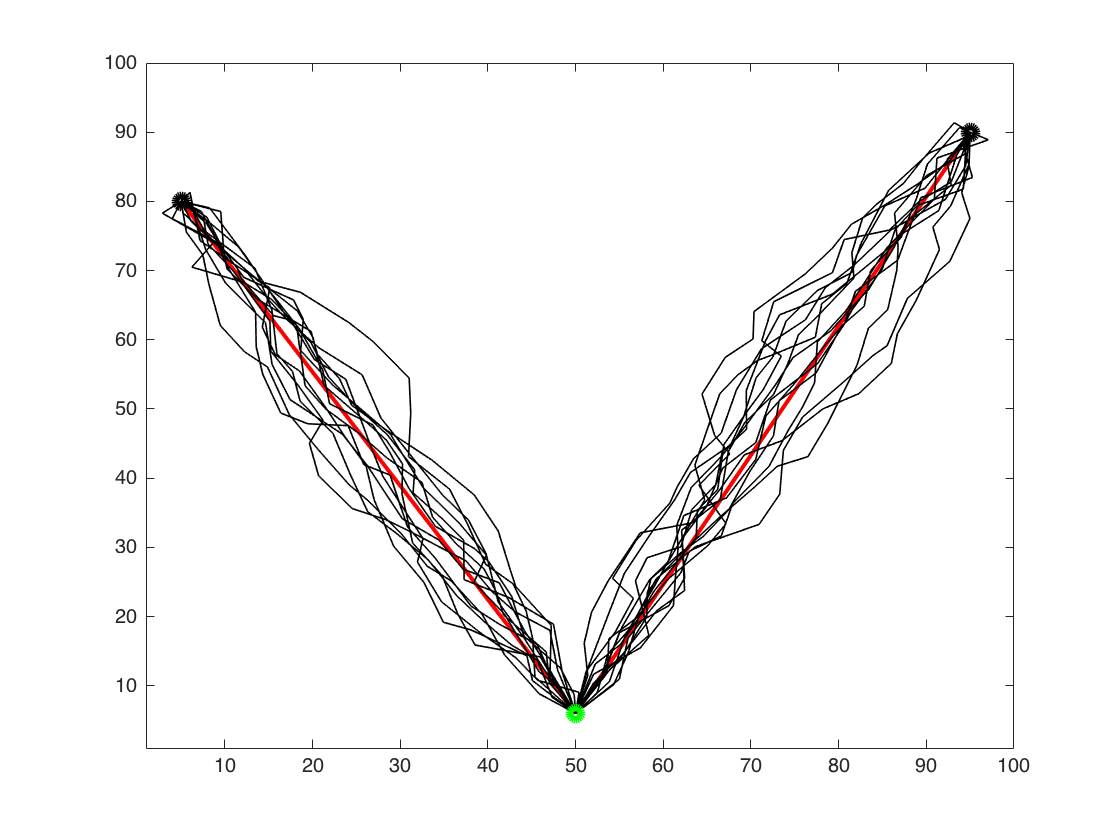
\includegraphics[width=0.8\linewidth]{figures/brownian_motion_mc.png}
	\ssp
	\caption{ Monte Carlo paths (black) surrounding deterministic N-NHV paths (red). The starting point, ($\vect{s} = [50 \ 6]^T$), is indicated in green. The set $K_N$ contains $N=2$ endpoints ($K_N = [ 5 \ 80 ]^T, [ 95 \ 90]^T$). $M_{mc}=15$ random walks are generated for each endpoint. $\alpha=5$. The variance of the Wiener process states are $\frac{1}{2} \alpha$.}

\end{figure}

% \begin{algorithm}[h!]
% \caption{Monte Carlo Path Planning (MCPP) with The Kriging Method}\label{alg:mcpp}
% \begin{algorithmic}[1]
% \Procedure{Kriging\_MCPP}{$Z$}
% 	\BState \emph{Conduct Initial Sweep}:
% 	\State SetWaypoint($[h\ w]^T$)
% 	\BState \emph{Krig The Field}:
% 	\State $\hat{Z}, \text{var}\{\hat{Z}\}$ = KrigingPredictField($Z$, $S$)

% 	\BState \textbf{while} $F > 0$ \textbf{and} $\Sigma_{\text{var}} > 0$:
% 	\State $P = []$
% 	\State $\Sigma_{\text{min}} = \infty$ \\

% 	\BState \ \ \ \ \emph{Find the highest field variances}:
% 	\State \ \ \ \ \textbf{for}\ $k = 1 \text{:} N$
% 	\State \ \ \ \  \ \ \ \ $S_{v}(k) = \argmax_{\vect{s}} \ \text{var}\{\hat{Z}_{k}(\vect{s})\}$
% 	\State \ \ \ \ \ \ \ \ $\text{var}\{\hat{Z}_{k+1}(\vect{s})\} = \text{var}\{\hat{Z}_{k}(\vect{s})\} - S_{v}(k)$\\

% 	\BState \ \ \ \  \emph{Calculate trajectories to all points found}:
% 	\State \ \ \ \  $\forall s_k \in S_{v}(k)$:
% 	\State \ \ \ \  \ \ \ \ $s_d = s_k$
% 	\State \ \ \ \  \ \ \ \ $f = \Big\lceil \frac{\|\vect{s}_c - \vect{s}_d\|_2}{\alpha} \Big\rceil$
% 	\State \ \ \ \  \ \ \ \ $T(1) = \begin{bmatrix} s_{c_x} \\ s_{c_y} \\ \text{arctan2}(s_{d_y} - s_{c_y}, s_{d_x} - s_{c_x}) \end{bmatrix}$
% 	\State \ \ \ \  \ \ \ \ $\forall i \in (1, f - 1)$:
% 	\State \ \ \ \  \ \ \ \  \ \ \ \ $T(i+1) = T(i) + \begin{bmatrix} \alpha \cos \theta(i) \\ \alpha \sin \theta(i) \\ \text{atan2}(s_{d_y} - T(i)_y, s_{d_x} - T(i)_x) \end{bmatrix} + \begin{bmatrix} \vect{w}(i) \\ 0 \end{bmatrix}$
% 	\State \ \ \ \  \ \ \ \ $T(f) = \begin{bmatrix} s_{d_x} \\ s_{d_y} \\ \theta_{f-1} \end{bmatrix}$\\

% 	\BState \ \ \ \  \ \ \ \  \emph{Calculate estimated field confidence for trajectory computed}:
% 	\State \ \ \ \  \ \ \ \  $\forall i \in [1, f]$:
% 	\State \ \ \ \  \ \ \ \  \ \ \ \ $\text{samples}(\hat{S}_T)$ += $\hat{Z}(T(i))$
% 	\State \ \ \ \  \ \ \ \  \ \ \ \ $\text{locations}(\hat{S}_T)$ += $T(i)$
% 	\State \ \ \ \  \ \ \ \  \ \ \ \ $\hat{Z}_T, \text{var}\{\hat{Z}\}_T$ = KrigingPredictField($Z$, $\hat{S}_T$)
% 	\State \ \ \ \  \ \ \ \  \ \ \ \ $\Sigma_{\text{var}}(T) = \text{avg}(\text{var}\{\hat{Z}\}_T)$\\

% 	\State \ \ \ \  \ \ \ \  \ \ \ \ \textbf{if} $\Sigma_{\text{var}}(T) < \Sigma_{\text{min}}$ \textbf{and} \text{length($T$)} $< F$:
% 	\State \ \ \ \  \ \ \ \  \ \ \ \ \ \ \ \ $\Sigma_{\text{min}} = \Sigma_{\text{var}}(T)$
% 	\State \ \ \ \  \ \ \ \  \ \ \ \ \ \ \ \ $P = T$\\

% 	\BState \ \ \ \  \emph{Navigate through the chosen path}:
% 	\State \ \ \ \  $\forall p \in P$:
% 	\State \ \ \ \  \ \ \ \ SetWaypoint($p$) 
% \EndProcedure
% \end{algorithmic}
% \end{algorithm}

% In Algorithm \ref{alg:mcpp}, the function \texttt{SetWaypoint()} is an abstracted function which steers the vehicle in the direction of the waypoint specified, and blocks the code instruction until the waypoint has been met. The function \texttt{length(}$T$\texttt{)} finds the arc length of the path by connecting all points in the trajectory, $T$. For a deterministically calculated trajectory, $T$, the arc length is $\alpha |T|$.

\begin{figure}[htb!]
	\centering
	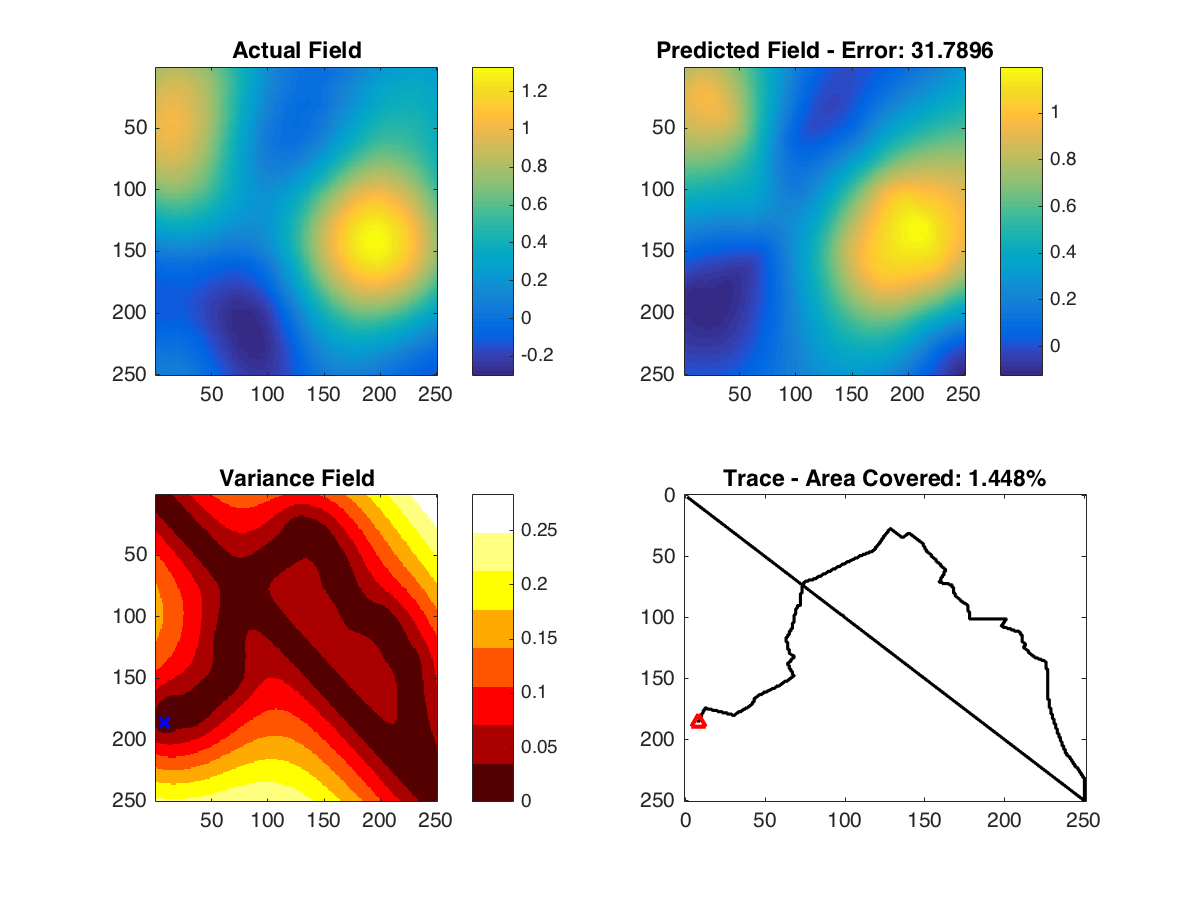
\includegraphics[width=0.95\linewidth]{figures/mc_4panel.png}
	\captionsetup{skip=0.20\baselineskip}
	\ssp
	\caption{The Monte Carlo Path Planner (MCPP) algorithm (Section \ref{sec:mcpp} terminated after two iterations of the algorithm. The actual field that is being explored is shown in the upper left. The current prediction of the actual field is shown in the upper right. The variance of the current prediction of the field is shown in the lower left. The trace of the exploration vehicle's path taken to the point of termination (in red) is shown in the lower right panel. All distance units are in meters. Here, $N$, the number of endpoints selected is $N=3$, and the number of random paths per cord calculated is $15$.}
	\label{fig:mcpp}
\end{figure}

\section{Planner Comparison}
The Monte Carlo based path planner (MCPP) takes into account a set of trajectories, and compares their estimated return on investment. The NHV simply takes the path to the high prediction uncertainty location. Though the MCPP algorithm, with a non-zero noise variance, does not deterministically calculate its trajectories, given enough trajectories, the algorithm could find a path that will reduce overall field uncertainty in a more brute-force way over the NHV algorithm. The disadvantages of The Monte Carlo Path Planner lay in the fact that the cost of each next move taken, are not considered directly. Rather, an entire trajectory is considered all at once. A more optimal approach to this planner would be to take into consideration the cost of each waypoint selected.
